\chapter{Typy vykreslení OSM dat}
\label{vykresleni_dat}

\begin{figure}[H]
    \centering
    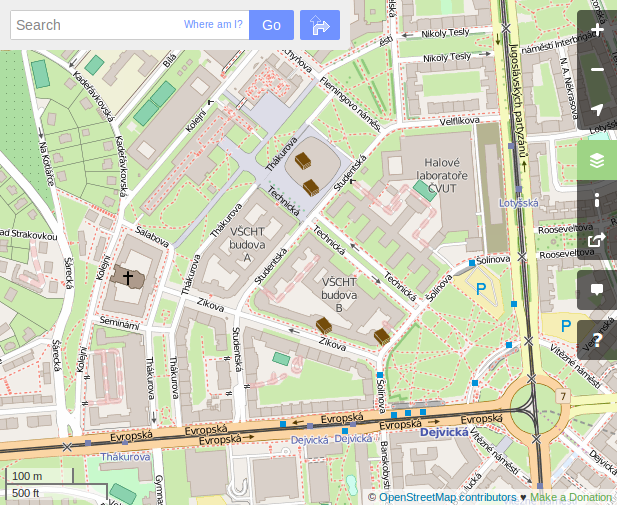
\includegraphics[width=11.5cm]{pictures/osm_standard.png} 
    \caption{Standardní mapa (Standard)}
    \label{fig:standard}
\end{figure}

\begin{figure}[H]
    \centering
    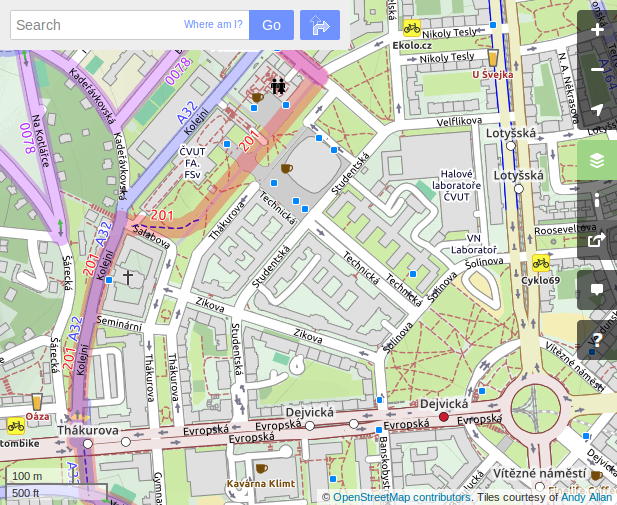
\includegraphics[width=11.5cm]{pictures/osm_cyclemap.png} 
    \caption{Cyklistická mapa (Cycle Map)}
    \label{fig:cycle}
\end{figure}

% new list

\begin{figure}[H]
    \centering
    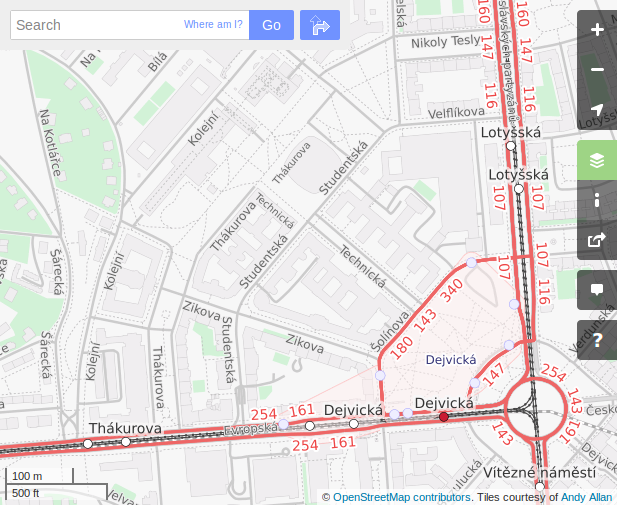
\includegraphics[width=11.5cm]{pictures/osm_transport.png} 
    \caption{Transport Map}
    \label{fig:transport}
\end{figure}

\begin{figure}[H]
    \centering
    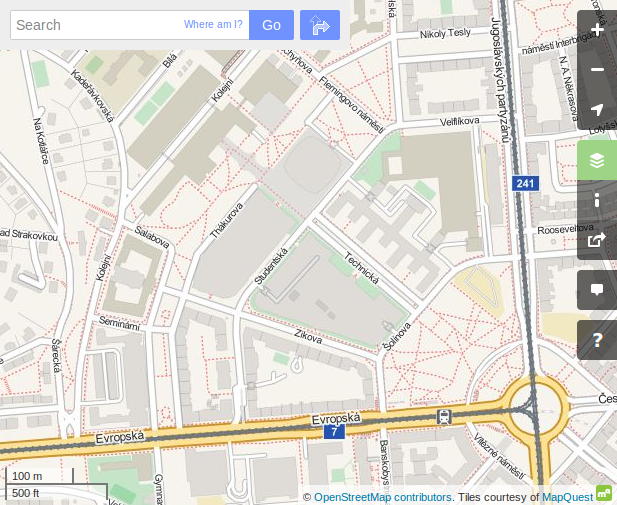
\includegraphics[width=11.5cm]{pictures/osm_mapquest.png} 
    \caption{MapQuest Open}
    \label{fig:mapquest}
\end{figure}

% new list

\begin{figure}[H]
    \centering
    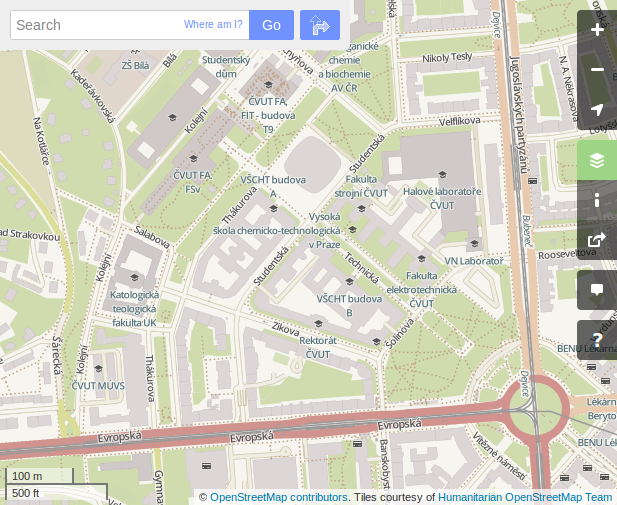
\includegraphics[width=11.5cm]{pictures/osm_humanitarian.png} 
    \caption{Humanitární mapa (Humanitarian)}
    \label{fig:humanitarian}
\end{figure}

\begin{figure}[H]
    \centering
    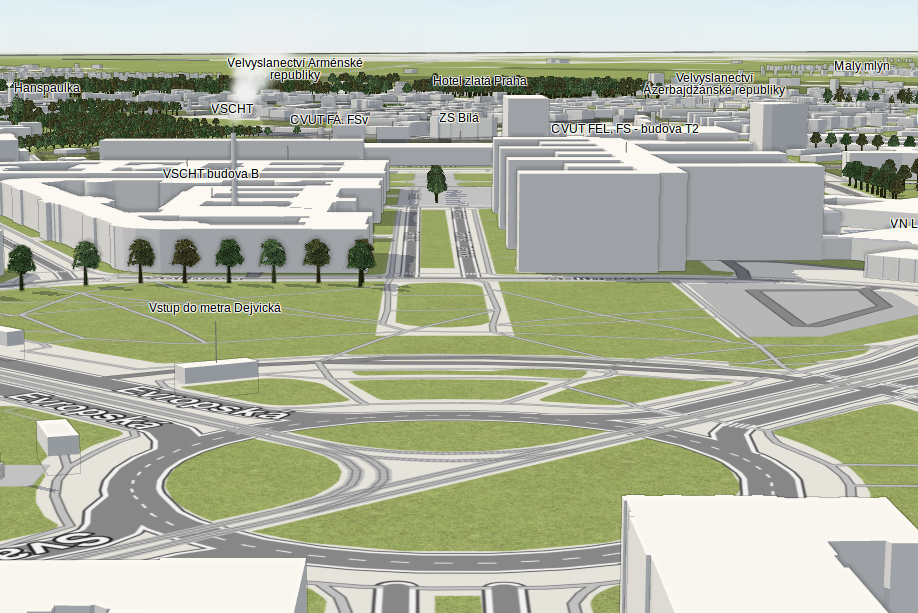
\includegraphics[width=11.5cm]{pictures/F4.png} 
    \caption{Projekt F4 (zdroj \url{http://demo.f4map.com/})}
    \label{fig:F4}
\end{figure}

% new list

\chapter{Diagramy}
\label{digramy}

\begin{figure}[H]
  \centering
  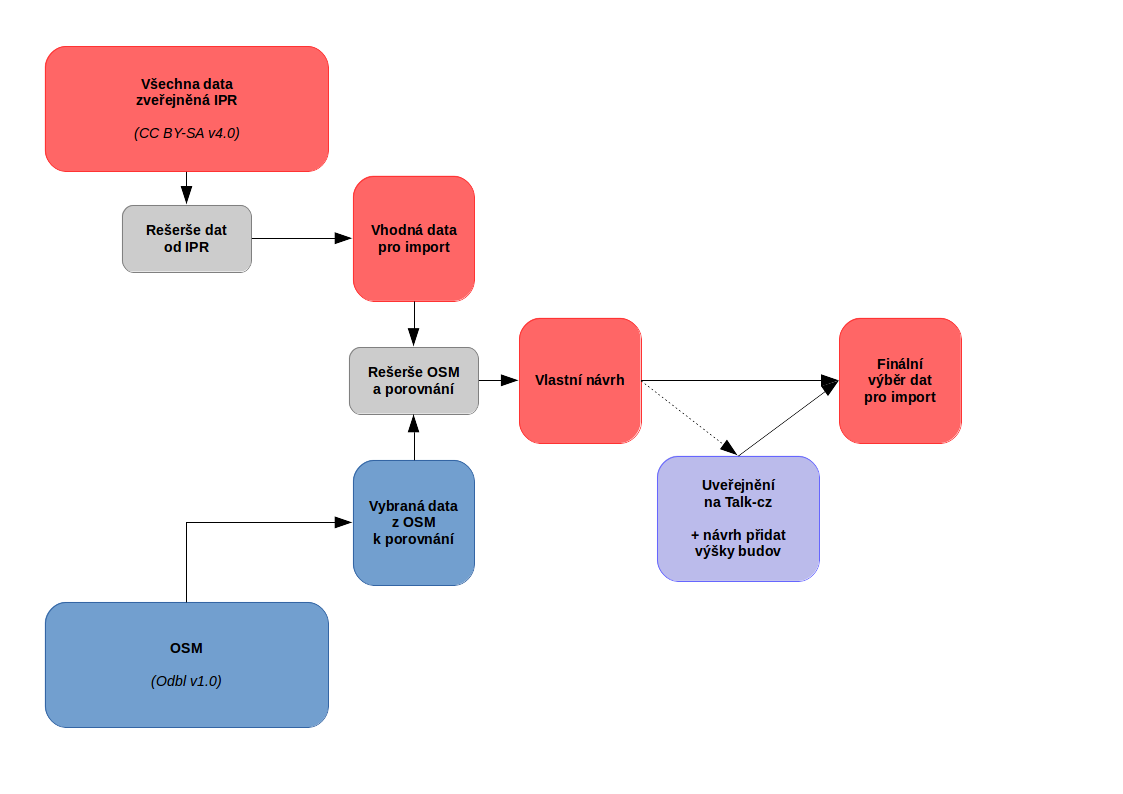
\includegraphics[scale=0.70,angle=90]{pictures/WorkFlow.png}
  \caption{Diagram postupu práce.}
  \label{fig:diagram_workflow}
\end{figure}

\begin{figure}[H]
  \centering
  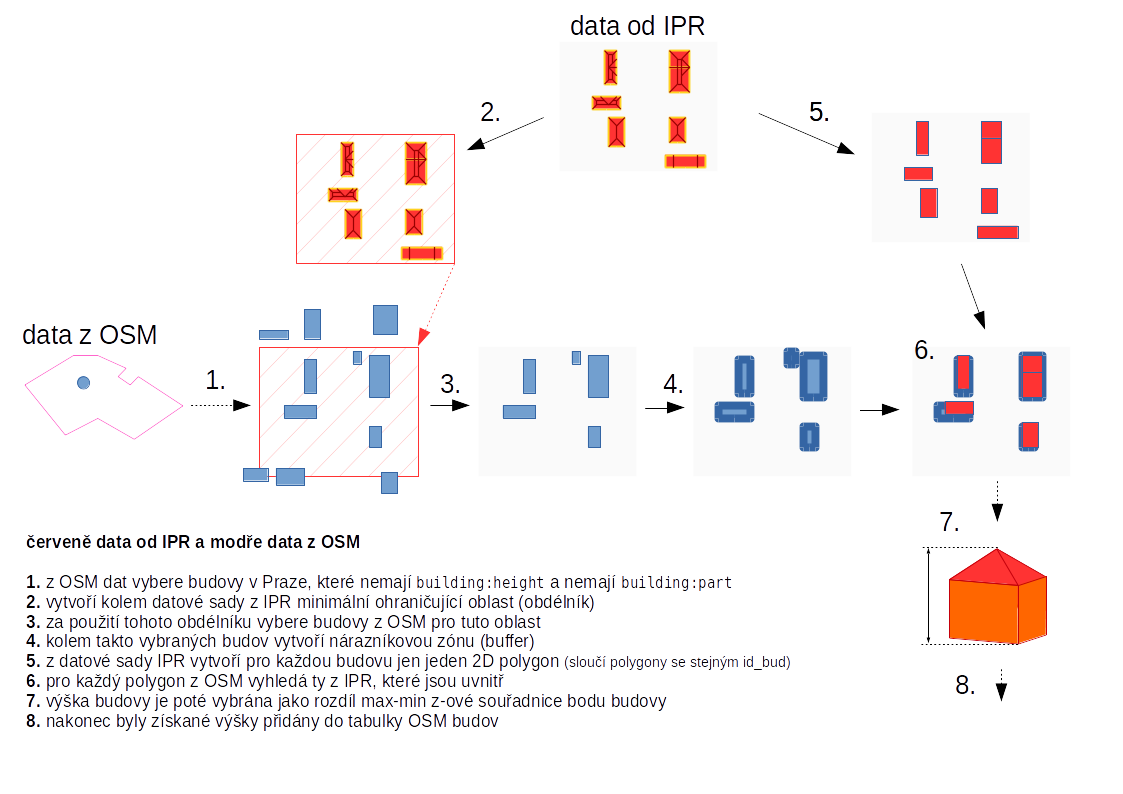
\includegraphics[scale=0.70,angle=90]{pictures/diagram_building_height.png}
  \caption{Diagram postupu práce pro získání výšky budov.}
  \label{fig:diagram_building}
\end{figure}

% new list

\chapter{Obsah CD}
\label{priloha-obsahCD}
\setlength{\unitlength}{.5mm}
\begin{picture}(250, 220)

  \put(  0, 212){\textbf{.}}

  \put(  1, 200){\line(0, 1){5}}
  \put(  1, 200){\line(1, 0){10} {\textbf{ src}}}  

      \put( 16, 190){\line(0, 1){8}}
      \put( 16, 190){\line(1, 0){10} {\textbf{ iprdownloader}}}
      \put(150, 190){ zdrojové soubory programu}

          \put( 29, 180){\line(0, 1){8}}
          \put( 29, 180){\line(1, 0){10} { IprBase.py}}
          \put( 29, 170){\line(0, 1){10}}
          \put( 29, 170){\line(1, 0){10} { IprPg.py}}
          \put( 29, 160){\line(0, 1){10}}
          \put( 29, 160){\line(1, 0){10} {\textbf{ Iprdownloader.py}}}

      \put( 16, 150){\line(0, 1){40}}
      \put( 16, 150){\line(1, 0){10} {\textbf{ pg}}}
      \put(150, 150){ zdrojové kódy shell skriptu}      

          \put( 29, 140){\line(0, 1){8}}
          \put( 29, 140){\line(1, 0){10} { pgis\_osm\_bp.style}}
          \put(150, 140){ vlastní schema dat z OSM}
          \put( 29, 130){\line(0, 1){10}}
          \put( 29, 130){\line(1, 0){10} { upgrade\_pgis\_osm\_bp.sql}}
          
      \put( 16, 120){\line(0, 1){30}}
      \put( 16, 120){\line(1, 0){10} {\textbf{ sql}}}
      \put(150, 120){ zdrojové kódy sql dump}
            
          \put( 29, 110){\line(0, 1){8}}
          \put( 29, 110){\line(1, 0){10} { buildins.sql}}
          \put( 29, 100){\line(0, 1){10}}
          \put( 29, 100){\line(1, 0){10} { park\_and\_ride.sql}}
          \put( 29,  90){\line(0, 1){10}}
          \put( 29,  90){\line(1, 0){10} { parkomat.sql}}
          \put( 29,  80){\line(0, 1){10}}
          \put( 29,  80){\line(1, 0){10} { recycling\_centre.sql}}
          \put( 29,  70){\line(0, 1){10}}
          \put( 29,  70){\line(1, 0){10} { toilets.sql}}          
          
  \put(  1,  60){\line(0, 1){140}}
  \put(  1,  60){\line(1, 0){10} {\textbf{ text}}}

      \put( 16,  50){\line(0, 1){8}}
      \put( 16,  50){\line(1, 0){10} {\textbf{ latex}}}
      \put(150,  50){ zdrojové soubory textu práce}
      \put( 16,  40){\line(0, 1){10}}
      \put( 16,  40){\line(1, 0){10} { martin-jakl-bp-2016.pdf}}
      \put(150,  40){ práce ve formátu PDF}
\end{picture}
